\documentclass[runningheads,a4paper]{llncs}

\usepackage{amssymb}
\setcounter{tocdepth}{3}
\usepackage{graphicx}
\usepackage{subfig}
\usepackage{url}
\usepackage{amsmath}
\usepackage{array}
\usepackage{booktabs}
%\urldef{\mailsa}\path|{alfred.hofmann, ursula.barth, ingrid.haas, frank.holzwarth,|
%\urldef{\mailsb}\path|anna.kramer, leonie.kunz, christine.reiss, nicole.sator,|
\urldef{\mailsc}\path|virk.shafqat@gmail.com, andycyrus@gmail.com, lwku@iis.sinica.edu.tw|    
\newcommand{\keywords}[1]{\par\addvspace\baselineskip
\noindent\keywordname\enspace\ignorespaces#1}

\begin{document}

\mainmatter  % start of an individual contribution

% first the title is needed
\title{Sinica Semantic Parser for ESWC'14 Concept-Level Semantic Analysis Challenge }

% a short form should be given in case it is too long for the running head
\titlerunning{Semantic Parsing}

% the name(s) of the author(s) follow(s) next
%
% NB: Chinese authors should write their first names(s) in front of
% their surnames. This ensures that the names appear correctly in
% the running heads and the author index.
%
\author{Shafqat Mumtaz Virk%
\and Yann-Huei Lee\and Lun-Wei Ku}
%
\authorrunning{Semantic Parsing}
% (feature abused for this document to repeat the title also on left hand pages)

% the affiliations are given next; don't give your e-mail address
% unless you accept that it will be published
\institute{Institute of Information Science (IIS)\\
Academia Sinica Taiwan\\
%\mailsa\\
%\mailsb\\
\mailsc\\
}

%
% NB: a more complex sample for affiliations and the mapping to the
% corresponding authors can be found in the file "llncs.dem"
% (search for the string "\mainmatter" where a contribution starts).
% "llncs.dem" accompanies the document class "llncs.cls".
%

%\toctitle{Lecture Notes in Computer Science}
%\tocauthor{Authors' Instructions}
\maketitle



\begin{abstract}
We present a semantic parsing system to decompose a sentence into semantic-expressions/concepts for ESWC'14 semantic analysis challenge. The proposed system has a pipeline architecture, and is based on syntactic parsing and semantic role labeling (SRL) of the candidate sentence. As to the former task, we use Stanford English parser; as to the later task, we use an in-house developed SRL system. The "concepts" are formulated from syntactically and semantically annotated sentences using a set of hand-build concept-formulation patterns. We also compare proposed system's performance to SenticNet with the help of few examples.
\keywords{Syntactic Parsing, Semantic Parsing, Semantic Role Labeling, Concept Formulation Templates}                 
\end{abstract}
\section{Introduction}
Natural languages are both complex and ambiguous. Unless machines are capable of handling these issues in an intelligent way, building smart natural language processing (NLP) applications is a tough and challenging task. Maybe, one way to ease this toughness is to try to make computers understand natural language text. For the same purpose, the trend in NLP is shifting from exploring 'what it is' to 'what it means' (i.e. from syntax to semantics). 

During the last couple of decades, a number of sub-fields have emerged under the umbrella term \textit{computational semantics}, and one such sub-field is \textit{semantic parsing}. This and many other such subfields (e.g. sentiment analysis, textual entailment, question answering, etc.) are among the rapidly growing sub-areas of NLP. The research community has recognized their worth and importance in recent times. This can be realized by the fact that their are many workshops, and special tracks/challenges in conferences, dedicated to these tasks. The ESWC'14 challenge on semantic analysis is one among those special challenges, and is scheduled to be held together with the 11th European Semantic Web Conference 2014 (ESWC'14). The challenge has a number of advanced tasks in addition to an elementary task on polarity detection. The advanced task\#2 is titled "Semantic Parsing", and refers to the task of de-constructing natural language text into a number of semantic-expressions/concepts. Though the term semantic-expression/concept is very general in itself, and is hard to define clearly, we take it to be a single-word/multi-word expression for which we have semantics.  


In this paper, we propose a system for \textit{semantic parsing} in the context of task\#2 of the challenge. The system has a pipeline architecture and relies on syntactic and semantic analysis of the candidate sentence. We use Stanford English parser \cite{stanford} for syntactic parsing, and an in-house developed semantic role labeling (SRL) system for semantic interpretations. To formulate the concepts into desired format, we propose a set of hand-build concept formulation templates. 
%The system takes a sentences as input and extract a number of and has a number of potential applications particularly in the fields of information retrieval, question answering, text summarization and machine translation. 
                
\section{Proposed System}
The architecture of the proposed system is shown in Fig.~\ref{fig:sys-archi}. It has three major components: a syntactic parsing, a semantic role labeling, and a concept formulation component. The purpose and importance of each component is explained in the following paragraphs.\\[0.3cm]
\begin{figure}[!h]
\centering
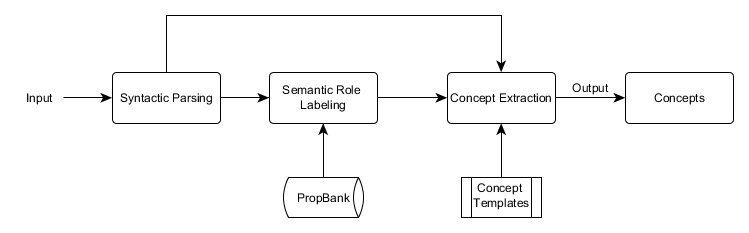
\includegraphics[width=.9\textwidth]{system-archi2.png}
\caption{System Architecture}
\label{fig:sys-archi}
\end{figure}
\textbf{Syntactic Parsing:} As a preliminary step, the input sentence is syntactically analyzed to get a syntactic parse tree. This step is necessary for the major reason that almost all automatic semantic role labeling system rely on a preliminary syntactic parsing step \cite{johansson}. \\[.3cm]
 %, (2) syntactic structure information may help to extract concepts in cases where the semantic role labeling does not help (more details are given in Section 3).
\textbf{Semantic Role Labeling:} Semantic role labeling (SRL), also known as shallow semantic parsing, is the task of semantically annotating natural language text. Conventionally, a syntactically parsed sentence is taken as input, and semantic arguments associated with predicate of the sentence are identified and classified to a particular semantic class. The first automatic semantic role labeling systems was reported by Gildea and Jurafsky in 2002 \cite{gildea}, and since then, their ideas have been dominating the field. In their approach, they emphasized on selection of appropriate lexical and syntactical features for SRL, use of statistical classifiers and their combinations, and ways to handle the data sparseness issue. Researchers have tried to build on that by augmenting and/or altering the feature set \cite{nianwen-2004}, by experimenting with various classification approaches \cite{pradan,park-2005}, and by attempting different ways to handle data sparseness \cite{zeprian}. For this challenge, we developed a SRL system, which is based largely on previously explored features and maximum entropy classifiers. The classifiers were trained using English Penn Treebank \cite{penn}, and Propbank \cite{propbank} data. However, we have proposed a number of additional features to enhance its performance. The details of the SRL system are beyond the scope of this paper, and are supposed to be covered in another planned article.  \\[0.3cm]   
%classes given in \cite{prop-guidlines}. Although we could not find an appropriate answer to the question "What a concept is?" from the  task of extracting concepts from natural language text requires a clear definition and a deep understanding of the term "concept" itself first, the predicates/verbs and their semantic components in a sentence are often good candidates. For the same reason, we take a syntactically parsed sentence and semantically annotate it using an in-house probabilistic semantic role labeling (SRL) system. The SRL system is based on many conventional features previously explored by \cite{gildea,pradan} and others, and a novel classification method. For the training purposes, we have used English Prop-Bank data \cite{propbank}. The details of the semantic role labeling are beyond the scope of this paper, and are supposed to be covered in another article. \\[0.3cm]
\textbf{Concept Formulation:} Once the sentence has been annotated syntactically and semantically, the concepts can be formulated using a set of hand-build concept templates. Table~\ref{tab:concept-template} lists few of the templates used in our experiments.
\begin{table}
\centering
\begin{tabular}{clcl}
\hline \textbf{\#} & \textbf{Concept Template} & \textbf{\#} & \textbf{Concept Template}\\ 
\hline 1  & ARG0\_Pred & 10  & Pred\_in\_the\_direction\_ARGM-DIR \\
\hline 2  & Pred\_ARG1  & 11  & Pred\_because\_ARGM-ARGM-CAU \\
\hline 3  & Pred\_ARG1\_ARG2 & 12  & Pred\_when\_ARGM-TMP \\
\hline 4 & Pred\_ARG1\_ARG2\_ARG3 & 13  & Pred\_ARGM-GOL \\ 
\hline 5 & Pred\_ARG1\_ARG2\_ARG3\_ARG4 & 14  & Pred\_by\_ARGM-EXT \\ 
\hline 6 & Pred\_ARG1\_ARG2\_ARG3\_ARG4\_ARG5 & 15 & Pred\_ARGM-MNR \\
\hline 7 & Pred\_with\_ARGM-COM & 16 &  Pred\_ARGM-NEG\\
\hline 8 & Pred\_in\_ARGM-LOC & 17 & ARGX's \\
\hline 9  & Pred\_in\_order\_to\_ARGM-PRP & 18 & ARGM's \\
\hline 
\end{tabular} 
\caption{Concept Templates}
\label{tab:concept-template}
\end{table}
Here, Pred and ARG1, ARG2, ARGM-LOC, ARGM-GOL, etc. refer to the predicate, and to the semantic role classes used in the prop-bank labeling scheme respectively (see \cite{prop-guidlines} for details on these classes). 

%Note that how the predicate of a sentence together with the semantic roles of its arguments are used to formulate semantic-expressions/concepts. An example follows in the next section.
%As an example, if we have the sentence \textit{'Pierre Vinken, 61 years old, will join the board as a non-executive director Nov. 29'}, the predicate 'join' has five semantic arguments: \{ ARG0:Pierre Vinken, 61 years old, ARG1:the board, ARGM-MOD:will, ARGM-PRD:as a non-executive director, ARGM-TMP:Nov. 29 \}. The predicate and its arguments can be used to extract the following semantic-expressions/concepts using the template given in \ref{tab:concept-template}.
%\begin{verbatim}
%{ Pierre Vinken , 61 years old ,_join
%join_the board
%will_join
%join_as a nonexecutive director
%join_{when}_Nov. 29}
%\end{verbatim}
%Since the coverage and performance of a SRL system can not guaranteed to be 100\%, largely because probabilistic systems have their limitations, syntactic information may provide  

\section{An Example} 
To explain how our proposed system works at different levels, lets take an example sentence: \textit{This film served as great entertainment for young people.}, and go through all the steps that the proposed system will perform to extract the semantic-expressions/concepts. As a first step the sentence will be syntactically parsed, which will be then semantically annotated by the SRL system. The resulting syntactically and semantically annotated tree is shown in Fig \ref{fig:parse-tree}.
\begin{figure}[!h]
\centering
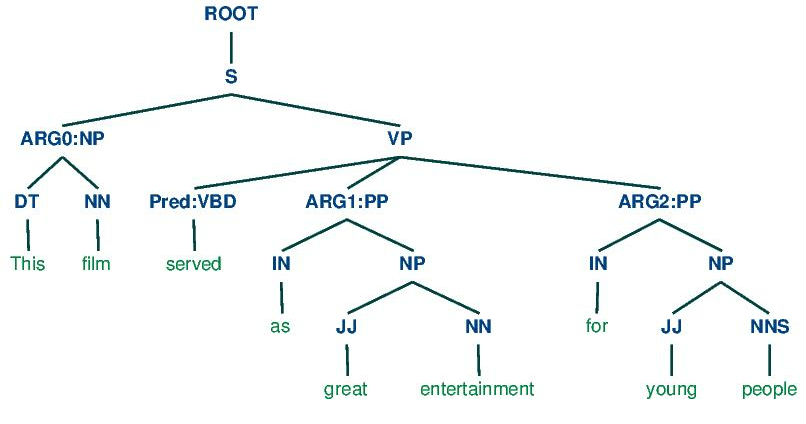
\includegraphics[width=.8\textwidth,height=5cm]{parse-tree6.jpg}
\caption{Syntactically and Semantically Annotated Parse Tree}
\label{fig:parse-tree}
\end{figure} 
From the semantically annotated tree, the extractable predicate-argument information is given in Table~\ref{tab:pred-arg-info}. Using this information and the templates given in Table~\ref{tab:concept-template}, the following concepts can be formulated:
\begin{verbatim}
(1) This_film_serve (2) serve_as_great_entertainment
(3) serve_for_young_people (4) great_entertainment
(5) This_film (6) young_people
\end{verbatim}
\begin{table}[!h]
\centering
\begin{tabular}{cp{10cm}}
\hline Predicate &  Arguments\\ 
\hline serve  & Arg0: This film \\
 & ARG1: as great entertainment \\
 & ARG2: for young people \\
\hline 
\end{tabular} 
\caption{Predicate-Argument Information}
\label{tab:pred-arg-info}
\end{table}    
\section{Comparison to SenticNet}
At the current stage of our experiments, we did not perform any automatic comparison or performance measurement leaving it to the official evaluation during the challenge days. However to give an idea to the reviewers, Table \ref{tab:sen-conc-compare} lists a couple of example sentences together with the extracted concepts both by the proposed system\footnote{A web-demo of the system is available at:}, and SenticNet\footnote{We used web-demo available at () to generate these concepts} \cite{senticnet}. We leave it to the reviewers to compare the outputs. 
\begin{table}[!h]
\centering
%\begin{tabular}{|p{2.5cm}|p{5.5cm}|p{3.8cm}|}
\begin{tabular}{>{\raggedright}p{3cm}>{\raggedright}p{5.5cm}p{3.5cm}<{\raggedright}}
\hline \textbf{Sentence} & \textbf{Proposed System's Output}  & \textbf{SenticNet's Output} \\ 
\hline I went to the market and bought fresh fruits and vegetables and came back &(1)bought\_fresh\_fruits (2)I\_went (3)I\_bought (4)vegetables (5)went\_to\_ the\_market (6)bought\_vegetables (7)fresh\_fruits (8)came\_\{in\_the\_direction\}\_ back (9)to\_the\_market (10)came\_I &(1)go\_to\_market (2)market (3)buy\_fruit (4)buy\_vegetable (5)fresh\_fruit (6)some\_fruit  (7)back\_come\\ 
\hline We also ordered the bedding and got the pillow & (1)got\_the\_pillow (2)the\_pillow (3)We\_got (4)the\_bedding (5)We\_order (7)order\_also (8)order\_the\_bedding & (1)also\_order (2)order\_bed (3)bed (4)get\_pillow (5)pillow \\ 
\hline 
\end{tabular}  
\caption{Example Sentences and Extracted Concepts}
\label{tab:sen-conc-compare}
\end{table}

%\begin{verbatim}
%(1)this_film (2) film_serv (3) great_entertain
%(4) serv_for_people (5) young_people
%\end{verbatim}

\subsection*{Acknowledgment}  
We would like to acknowledge that this work was partially supported by National Science Council, Taiwan, under the contract NSC 102-2221-E-001-026.
%\begin{figure}[htbp]
%\centering
%\subfloat{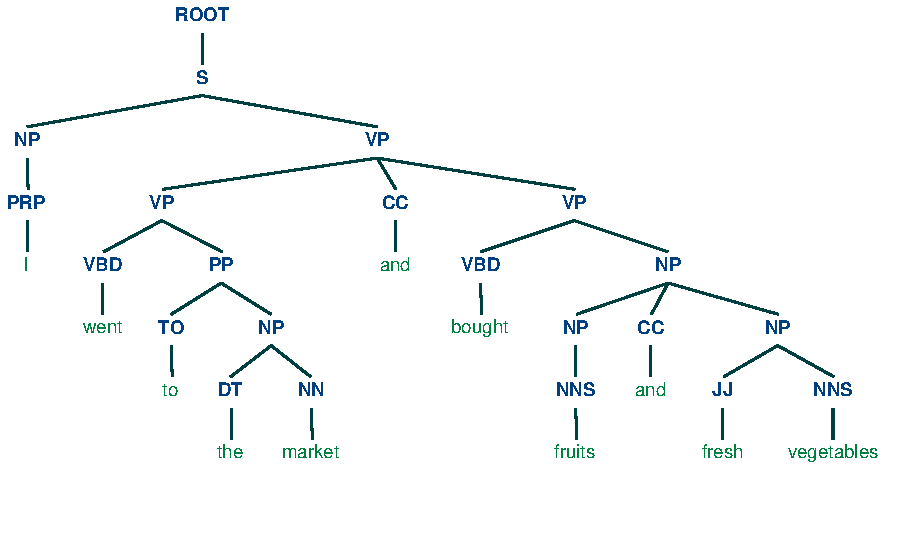
\includegraphics[height=3.5cm]{parse-tree2.pdf}}\hfill
%\subfloat{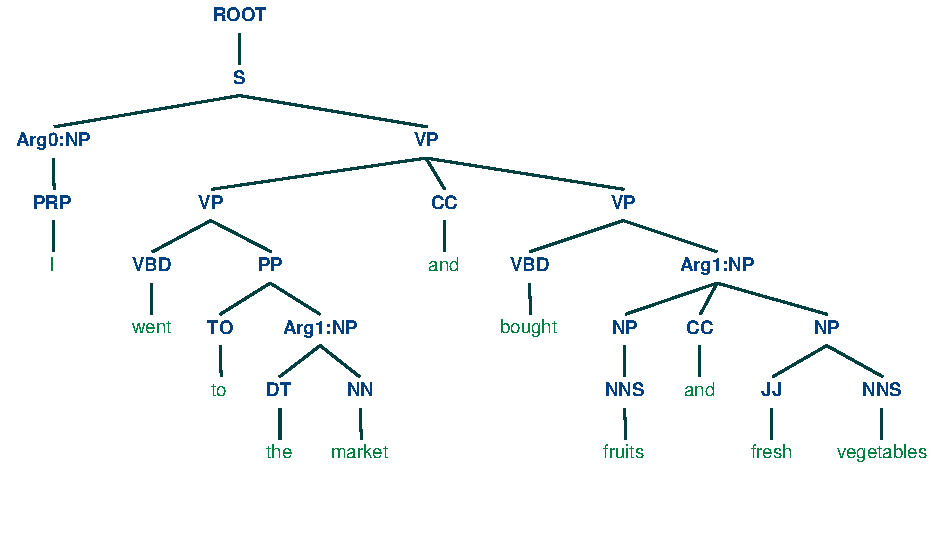
\includegraphics[height=3.5cm]{srl-tree.pdf} }\\
%\caption{(a) Parse Tree \hspace{3cm}   (b) Semantically Annotated Tree}
%\label{fig:parse-trees}
%\end{figure}
%\section{Testing and evaluation}
%We selected 6037 random sentences from English PennTreebank \cite{penn}, and the corresponding Propbank \cite{propbank} data for testing and evaluation purposes. As mentioned previously, we build two systems. In the system 'Sys-SP', each input sentence is parsed using Stanford English parser, and the concepts are extracted using concept-extracting pattern given in table~\ref{tab:concept-template}. In the system 'Sys-SRL', the syntactically and semantically pre-parsed sentences (i.e. Penn Treebank and Propbank data) are used to extract the concepts with the help of concept-extracting patterns given in Table~\ref{tab:concept-template}. In both the systems, we also extract concepts from complex noun-phrases. Statistics about the number of extracted, and the source of the concepts for each system are given in Table~\ref{tab:concept-stats} .
%\begin{table}[h!]
%\centering
%\begin{tabular}{|l|c|c|}
%\hline \textbf{Round/Stats} & \textbf{Sys-SP} & \textbf{Sys-SRL}  \\ 
%\hline \#Sentences & 6037  & 6037 \\ 
%\hline \# Pred-Arg Concepts & 21811 & 10025 \\ 
%\hline \# Complex-NP Concepts & 34725 & 54188  \\ 
%\hline \ Total \# Concepts & 56536  &  64213\\ 
%\hline Avg concepts/sentence & 9.36 & 10.6 \\ 
%\hline 
%\end{tabular} 
%\caption{Results}
%\label{tab:concept-stats}
%\end{table} 

%It is worth pointing out that in the real system (the one which will be used in the open challenge), the syntactic parsing and semantic role labeling will be done using Stanford English parser and an in-house semantic role labeler respectively. The reason for not involving these two components in the current experiment is the time limitation that we have to conduct the experiments and submit the paper. 


%Since the test/evaluation data set is not released at this stage, and we are not sure how the proposed system will be evaluated, we evaluate our proposed systems by simply comparing the number of concepts produces per sentence. The results for a small set of 100 sentences are given in Table~\ref{tab:eval-results}. A better evaluation might have involved human evaluators to compare the quality of concepts produces by each of the three systems, but due to the time constraints, we are unable to do that kind of evaluation at this stage.
%\begin{table}[h!]
%\centering
%\begin{tabular}{|l|c|c|}
%\hline \textbf{SentiNet} & \textbf{Sys-SP} & \textbf{Sys-SRL}  \\ 
%\hline  &  &  \\ 
%\hline 
%\end{tabular} 
%\caption{Results}
%\label{tab:eval-results}
%\end{table}       
%To evaluate the performance of our proposed systems, we compare their output to the output produced by SentiNet. For a small set of 100 sentences, three sets of concepts are produced using 'Sys-SP', 'Sys-SRL', and 'SentiNet'. An human evaluator then compares their performance. The comparison method is as: For each concept generated by 'SentiNet', if the same concept is generated by any of the proposed system (i.e. 'Sys-SP' or 'Sys-SRL'), the proposed system gets one point. This process is repeated for each of the 100 test sentences. Additional, if the proposed system generates an additional concept, which the human evaluator considers to be useful, the proposed system gets an extra point. Similarly, the proposed system gets a penalty of one point for every useless generated concept. Considering the fact that no standard evaluation parameters/methods were suggested by the challenge organizers, nor any evaluation and/or test data was given, we propose the above mentioned evaluation method. The evaluation results for 100 test sentences are given in Table N.     

\begin{thebibliography}{4}
\bibitem{zeprian} Be\'{n}at Zapirain and Eneko Agirre and Llu\'{\i}s M\`{a}rquez. Ubc-upc: Sequential srl using selectional preferences: An aproach with maximum entropy markov models. In Proceedings of the 4th International Workshop on Semantic Evaluations, pages 354-357, Stroudsburg, PA, USA. Association for Computational Linguistics. 2007.
\bibitem{prop-guidlines} Claire Bonial, Jena Hwang, Julia Bonn, Kathryn Conger, Olga Babko-Malaya and Martha Palmer, English PropBank Annotation Guidelines, Center for Computational Language and Education Research Institute of Cognitive Science University of Colorado at Boulder, Nov, 2012.
\bibitem{stanford} Dan Klein and Christopher D. Manning. Accurate Unlexicalized Parsing. Proceedings of the 41st Meeting of the Association for Computational Linguistics, pp. 423-430, 2003.
\bibitem{senticnet} Erik Cambria, Daniel Olsher, Dheeraj Rajagopal. SenticNet 3: A Common and Common-Sense Knowledge Base for Cognition-Driven Sentiment Analysis, Association for the Advancement of Artificial Intelligence. 2014. 
\bibitem{gildea} Gildea Daniel and Daniel Jurafsky. Automatic labeling of semantic roles. Computational Linguistics, 28(3): 245-288, 2002.
\bibitem{park-2005} Kyung-Mi Park and Hae-Chang Rim. Maximum entropy based semantic role labeling. In Proceedings of the Ninth Conference on Computational Natural Language Learning, CONLL ?05, pages 209-212, Stroudsburg, PA, USA. Association for Computational Linguistics, 2005.
\bibitem{propbank} Martha Palmer, Dan Gildea, Paul Kingsbury, The Proposition Bank: A Corpus Annotated with Semantic Roles, Computational Linguistics Journal, 31:1, 2005.
\bibitem{penn} Mitchell P., Beatrice Santorini and Mary Ann Marcinkiewicz, Building a Large Annotated Corpus of English: The Penn Treebank: COMPUTATIONAL LINGUISTICS, 10(2), pages 313-330, 1993.
\bibitem{nianwen-2004} Nianwen Xue. Calibrating features for semantic role labeling. In Proceedings of EMNLP 2004, pages 88-94. 2004.
\bibitem{johansson} Richard Johansson and Pierre Nuges, The Effect of Syntactic Representation on Semantic Role Labeling, Proceedings of the 22nd International Conference on Computational Linguistics (Coling 2008), pages 393-400, Manchester, August 2008.
\bibitem{pradan} Sammer Pradhan, Wayne Ward, Kadri Haciuglu, James Martin, and Dan Jurafsky. 2004. Shallow semantic parsing using support vector machines. In Proceedings of HLT/NAACL-2004

%\bibitem{framenet} Collin F. Baker, Charles J. Fillmore and John B. Lowe, The Berkeley FrameNet Project, International Computer Science Institute 1947 Center St. Suite 600 Berkeley, Calif., 94704.

\end{thebibliography}
\end{document}